% GNUPLOT: LaTeX picture with Postscript
\begingroup
  \makeatletter
  \providecommand\color[2][]{%
    \GenericError{(gnuplot) \space\space\space\@spaces}{%
      Package color not loaded in conjunction with
      terminal option `colourtext'%
    }{See the gnuplot documentation for explanation.%
    }{Either use 'blacktext' in gnuplot or load the package
      color.sty in LaTeX.}%
    \renewcommand\color[2][]{}%
  }%
  \providecommand\includegraphics[2][]{%
    \GenericError{(gnuplot) \space\space\space\@spaces}{%
      Package graphicx or graphics not loaded%
    }{See the gnuplot documentation for explanation.%
    }{The gnuplot epslatex terminal needs graphicx.sty or graphics.sty.}%
    \renewcommand\includegraphics[2][]{}%
  }%
  \providecommand\rotatebox[2]{#2}%
  \@ifundefined{ifGPcolor}{%
    \newif\ifGPcolor
    \GPcolorfalse
  }{}%
  \@ifundefined{ifGPblacktext}{%
    \newif\ifGPblacktext
    \GPblacktexttrue
  }{}%
  % define a \g@addto@macro without @ in the name:
  \let\gplgaddtomacro\g@addto@macro
  % define empty templates for all commands taking text:
  \gdef\gplbacktext{}%
  \gdef\gplfronttext{}%
  \makeatother
  \ifGPblacktext
    % no textcolor at all
    \def\colorrgb#1{}%
    \def\colorgray#1{}%
  \else
    % gray or color?
    \ifGPcolor
      \def\colorrgb#1{\color[rgb]{#1}}%
      \def\colorgray#1{\color[gray]{#1}}%
      \expandafter\def\csname LTw\endcsname{\color{white}}%
      \expandafter\def\csname LTb\endcsname{\color{black}}%
      \expandafter\def\csname LTa\endcsname{\color{black}}%
      \expandafter\def\csname LT0\endcsname{\color[rgb]{1,0,0}}%
      \expandafter\def\csname LT1\endcsname{\color[rgb]{0,1,0}}%
      \expandafter\def\csname LT2\endcsname{\color[rgb]{0,0,1}}%
      \expandafter\def\csname LT3\endcsname{\color[rgb]{1,0,1}}%
      \expandafter\def\csname LT4\endcsname{\color[rgb]{0,1,1}}%
      \expandafter\def\csname LT5\endcsname{\color[rgb]{1,1,0}}%
      \expandafter\def\csname LT6\endcsname{\color[rgb]{0,0,0}}%
      \expandafter\def\csname LT7\endcsname{\color[rgb]{1,0.3,0}}%
      \expandafter\def\csname LT8\endcsname{\color[rgb]{0.5,0.5,0.5}}%
    \else
      % gray
      \def\colorrgb#1{\color{black}}%
      \def\colorgray#1{\color[gray]{#1}}%
      \expandafter\def\csname LTw\endcsname{\color{white}}%
      \expandafter\def\csname LTb\endcsname{\color{black}}%
      \expandafter\def\csname LTa\endcsname{\color{black}}%
      \expandafter\def\csname LT0\endcsname{\color{black}}%
      \expandafter\def\csname LT1\endcsname{\color{black}}%
      \expandafter\def\csname LT2\endcsname{\color{black}}%
      \expandafter\def\csname LT3\endcsname{\color{black}}%
      \expandafter\def\csname LT4\endcsname{\color{black}}%
      \expandafter\def\csname LT5\endcsname{\color{black}}%
      \expandafter\def\csname LT6\endcsname{\color{black}}%
      \expandafter\def\csname LT7\endcsname{\color{black}}%
      \expandafter\def\csname LT8\endcsname{\color{black}}%
    \fi
  \fi
  \setlength{\unitlength}{0.0500bp}%
  \begin{picture}(8502.00,5102.00)%
    \gplgaddtomacro\gplbacktext{%
      \csname LTb\endcsname%
      \put(946,704){\makebox(0,0)[r]{\strut{}1978}}%
      \put(946,1171){\makebox(0,0)[r]{\strut{}1978}}%
      \put(946,1638){\makebox(0,0)[r]{\strut{}1978}}%
      \put(946,2105){\makebox(0,0)[r]{\strut{}1979}}%
      \put(946,2573){\makebox(0,0)[r]{\strut{}1980}}%
      \put(946,3040){\makebox(0,0)[r]{\strut{}1980}}%
      \put(946,3507){\makebox(0,0)[r]{\strut{}1980}}%
      \put(946,3974){\makebox(0,0)[r]{\strut{}1981}}%
      \put(946,4441){\makebox(0,0)[r]{\strut{}1982}}%
      \put(1078,484){\makebox(0,0){\strut{}-166}}%
      \put(2249,484){\makebox(0,0){\strut{}-164}}%
      \put(3420,484){\makebox(0,0){\strut{}-162}}%
      \put(4592,484){\makebox(0,0){\strut{}-160}}%
      \put(5763,484){\makebox(0,0){\strut{}-158}}%
      \put(6934,484){\makebox(0,0){\strut{}-156}}%
      \put(8105,484){\makebox(0,0){\strut{}-154}}%
      \put(176,2572){\rotatebox{-270}{\makebox(0,0){\strut{}$T \ [ms]$}}}%
      \put(4591,154){\makebox(0,0){\strut{}$x \ [mm]$}}%
      \put(4591,4771){\makebox(0,0){\strut{}Vermessung negativer Schnittpunkt von $T_A(x)$ und $T_B(x)$}}%
    }%
    \gplgaddtomacro\gplfronttext{%
      \csname LTb\endcsname%
      \put(7118,4268){\makebox(0,0)[r]{\strut{}Messwerte $T_A(x)$}}%
      \csname LTb\endcsname%
      \put(7118,4048){\makebox(0,0)[r]{\strut{}Messwerte $T_B(x)$}}%
      \csname LTb\endcsname%
      \put(7118,3828){\makebox(0,0)[r]{\strut{}$f(x) = ax+b$}}%
      \csname LTb\endcsname%
      \put(7118,3608){\makebox(0,0)[r]{\strut{}$g(x) = cx+d$}}%
    }%
    \gplbacktext
    \put(0,0){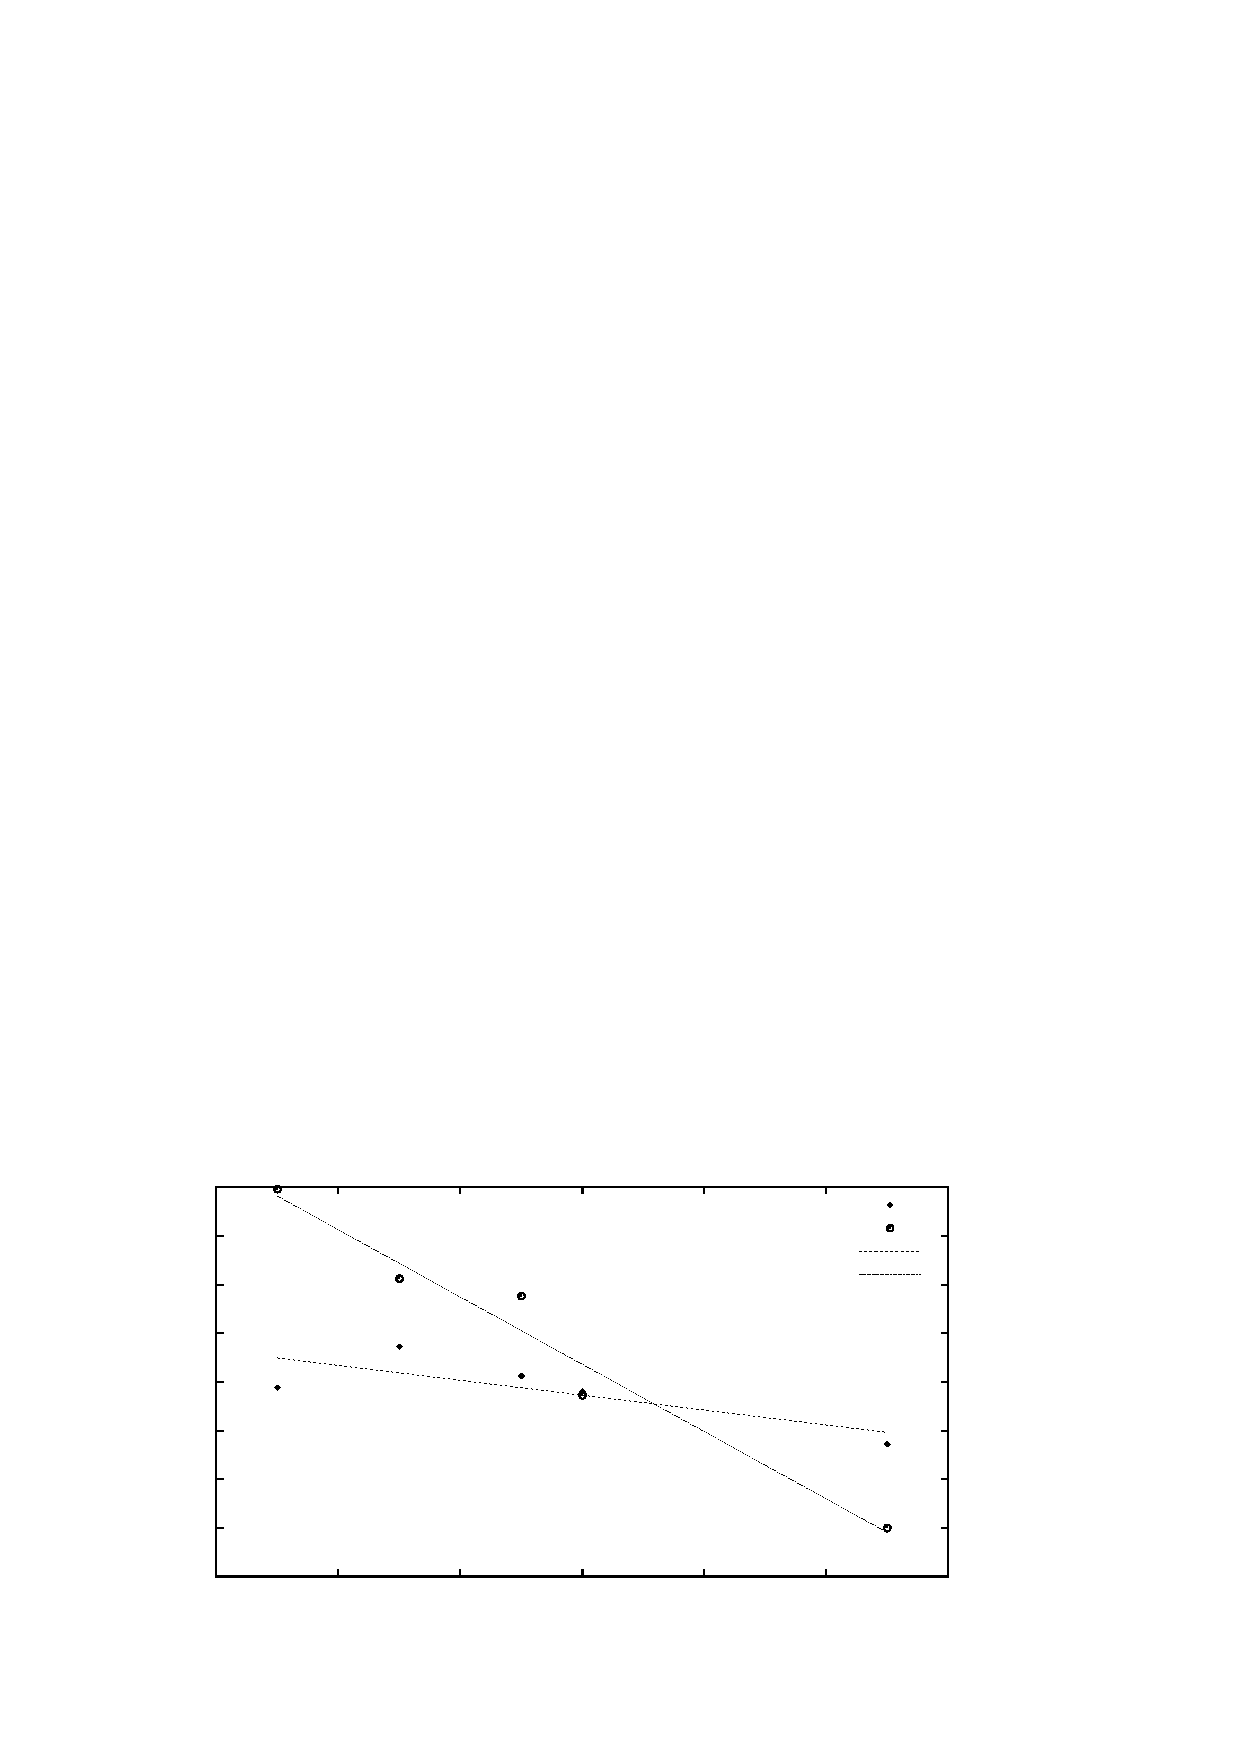
\includegraphics{TA-TB-x-fein-n}}%
    \gplfronttext
  \end{picture}%
\endgroup
